\section{Exp3: Pushing task in simulation I}
\label{sec:push_sim_1}

The next task was to push a square cube into some target position using
the real robot arm, however preliminary experiments using NAF did not
converge to an intuitively good policy. Instead of rejecting the capabilities
of the NAF algorithm at this stage, simulation experiments were first done in
a more ideally set up environment.

\subsection{Environment}

The environment consisted of a circular object to push into some goal position.
To simplify the problem, these locations were sampled approximately at the same
position at every reset. This was in order to ignore rotations and translations
of the problem and only examine whether the algorithm could learn this simpler
scenario. The simulated end-effector was a single point and was sampled
uniformly in the entire workspace. The reward was defined as $e^{-k_1 ||\mathbf{e
- c}||} + e^{-k_2 ||\mathbf{c - g}||}$ where $\mathbf{e, c}$ and $\mathbf{g}$
are the poses of the end-effector, the pushable circle, and the goal
position.

\subsection{Algorithms}

The NAF algorithm was used where the network consisted of 2 hidden layers of
200 ReLU activated units each. The activation function for the $\mu$ output was
a tanh-function scaled by $0.01$. A prioritized experience replay buffer was
used to store and sample mini batches of size $64$. Samples were drawn with
probability proportional to $p_i = |\delta_i| + \epsilon|$ where $\delta_i$ is
the latest temporal difference error of sample $i$ and $\epsilon = 10^{-9}$.
The loss for each sample $i$ was scaled by using importance sampling weights
$\left( \frac{1}{p_i}\right) ^\beta$ where $\beta$ was linearly annealed from
$0$ to $1$. A decay factor $\gamma = 0.99$ was used.

\subsection{Results}

The algorithm was able to approach the pushable object, but unable to push it
to the target position including going around the object to push it towards the
target. This is illustrated in figure \ref{fig:naf_sim_failure}. In figure
\ref{fig:naf_sim_unimode_q}, the Q-function is shown for a scenario where
intuitively the optimal policy should be to go up or down, but not left or
right. It is unclear if this is due to the quadratic shape of the advantage
function being unable to represent this, or some other detail in the
implementation.

\begin{figure}[h!]
    \centering
    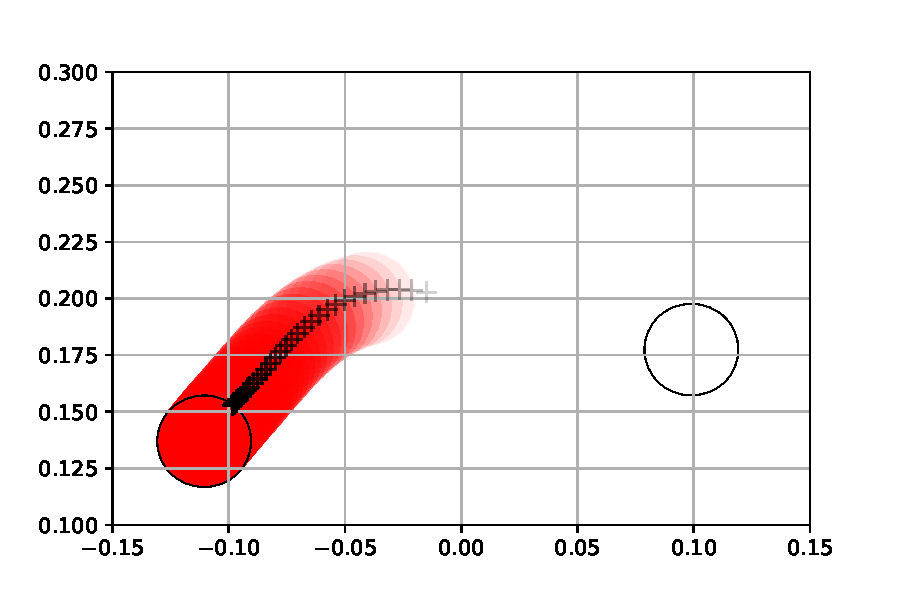
\includegraphics[width=0.4 \textwidth]{res/naf_sim_failure_mode.pdf}
    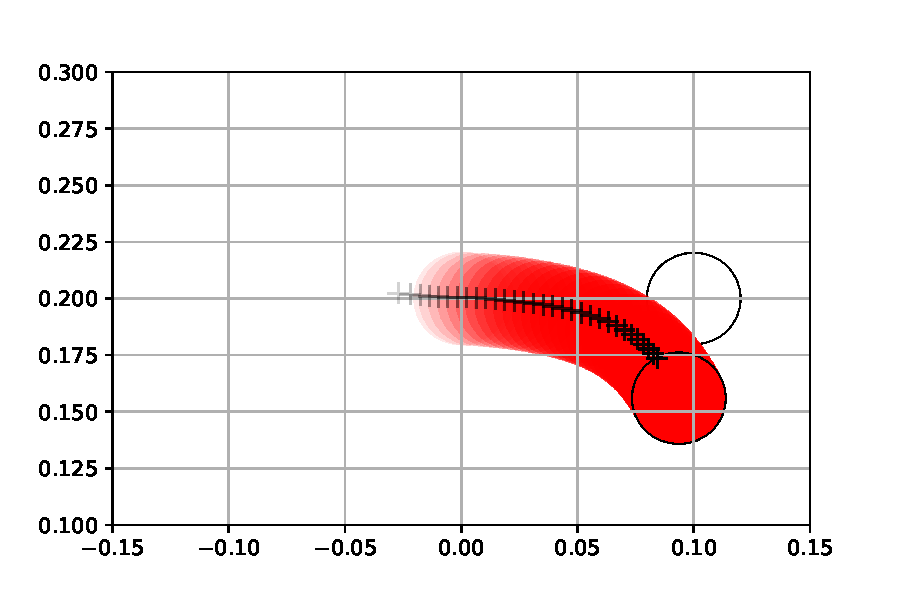
\includegraphics[width=0.4 \textwidth]{res/naf_sim_failure_mode_ideal.pdf}

    \caption{Results of NAF in simulation on pushing task. The red circle is
    the object being pushed, the white circle is the goal, and the cross is the
    simulated end-effector.}

    \label{fig:naf_sim_failure}
\end{figure}

\begin{figure}[h!]
    \centering
    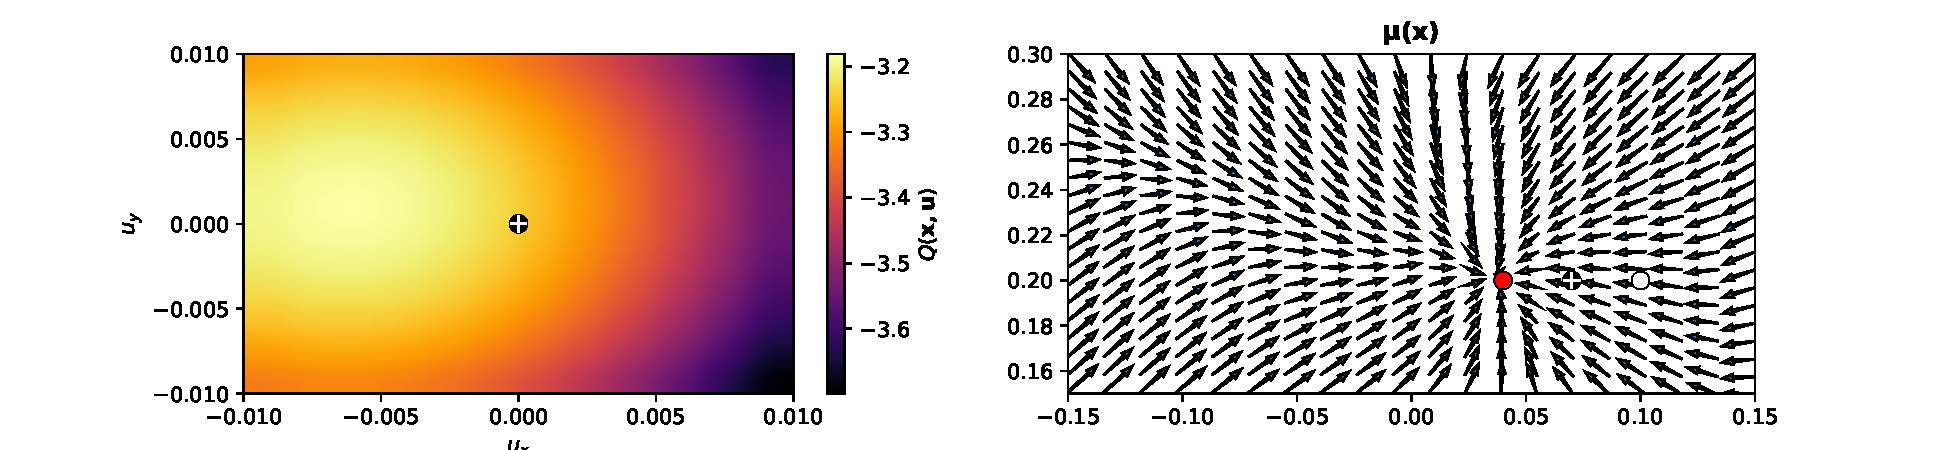
\includegraphics[width=1.0 \textwidth]{res/naf_sim_unimode_q.pdf}

    \caption{Results from using NAF on a simulated pushing task. Q-function and
    policy of the state given by the pushable object (red), the goal (white
    circle), and the end-effector (white cross). Since the advantage function
    is parameterized by a quadratic expression, which is uni-modal, the
    Q-function cannot represent the bi-modal nature of this scenario.}

    \label{fig:naf_sim_unimode_q}
\end{figure}
